\section{Introduction}\label{sec:Introduction}
This technote is a first evaluation of the potential of the MicroBooNE Cosmic Ray Tagger (CRT) in electron neutrino searches using MicroBooNE data.  In section \ref{sec:Stability} of this note, we discuss the stability of the CRT system and the amount of  currently available POTs collected with CRT data usable for physics analyses. In section \ref{sec:Cuts}, we describe two cuts -- the CRT Veto $\nu_e$overlayand the CRT Distance Tagger -- that can be used in  the  preselection for $\nu_e$ searches. The rejection power and signal efficiency of these cuts is evaluated in section \ref{sec:RejectionAndEff}. In section \ref{sec:Significance}, we draw a first comparison of the selection significance for the Cutflow with and without the use of CRT information. We summarize the highlights and take-aways of this note in section \ref{sec:Conclusions}. 

\section{Good CRT Data and CRT Stability}\label{sec:Stability}
When fully functional, the MicroBooNE Cosmic Ray Tagger system counts a total of 73 modules, shown in figure \ref{fig:CRT} and distributed as follows: 9 modules on two layers for the bottom panel (cyan and blue in the figure), 13 modules on two layers for the feedthrough side panel (yellow and cyan),  27 modules on three layers for the pipe side panel (pink, orange and light blue),  24 modules on two layers for the top panel (green and blue).  The installation of the bottom and sides panels took place in the summer of 2016, while the installation of the top panel tool place in February 2017. 
The CRT data is recorded and stored with a stand alone data acquisition system external to the MicroBooNE main DAQ. The CRT data is then merged to the PMT and TPC data offline at swizzling time; the data merger uses the CRT and TPC independently recorded GPS timestamps to match the CRT and TPC events. A hardware issue with the CRT GPS timestamp distribution was discovered and fixed on November 30th 2017 (see elog entry 60189). That elog entry highlights that the first TPC run number with matchable CRT information is run 14114.  We note here that more work would be necessary to try to recover CRT data between Feb 2017 and Nov 2017 with no guarantee of success. 


\begin{figure}[h!]
\centering
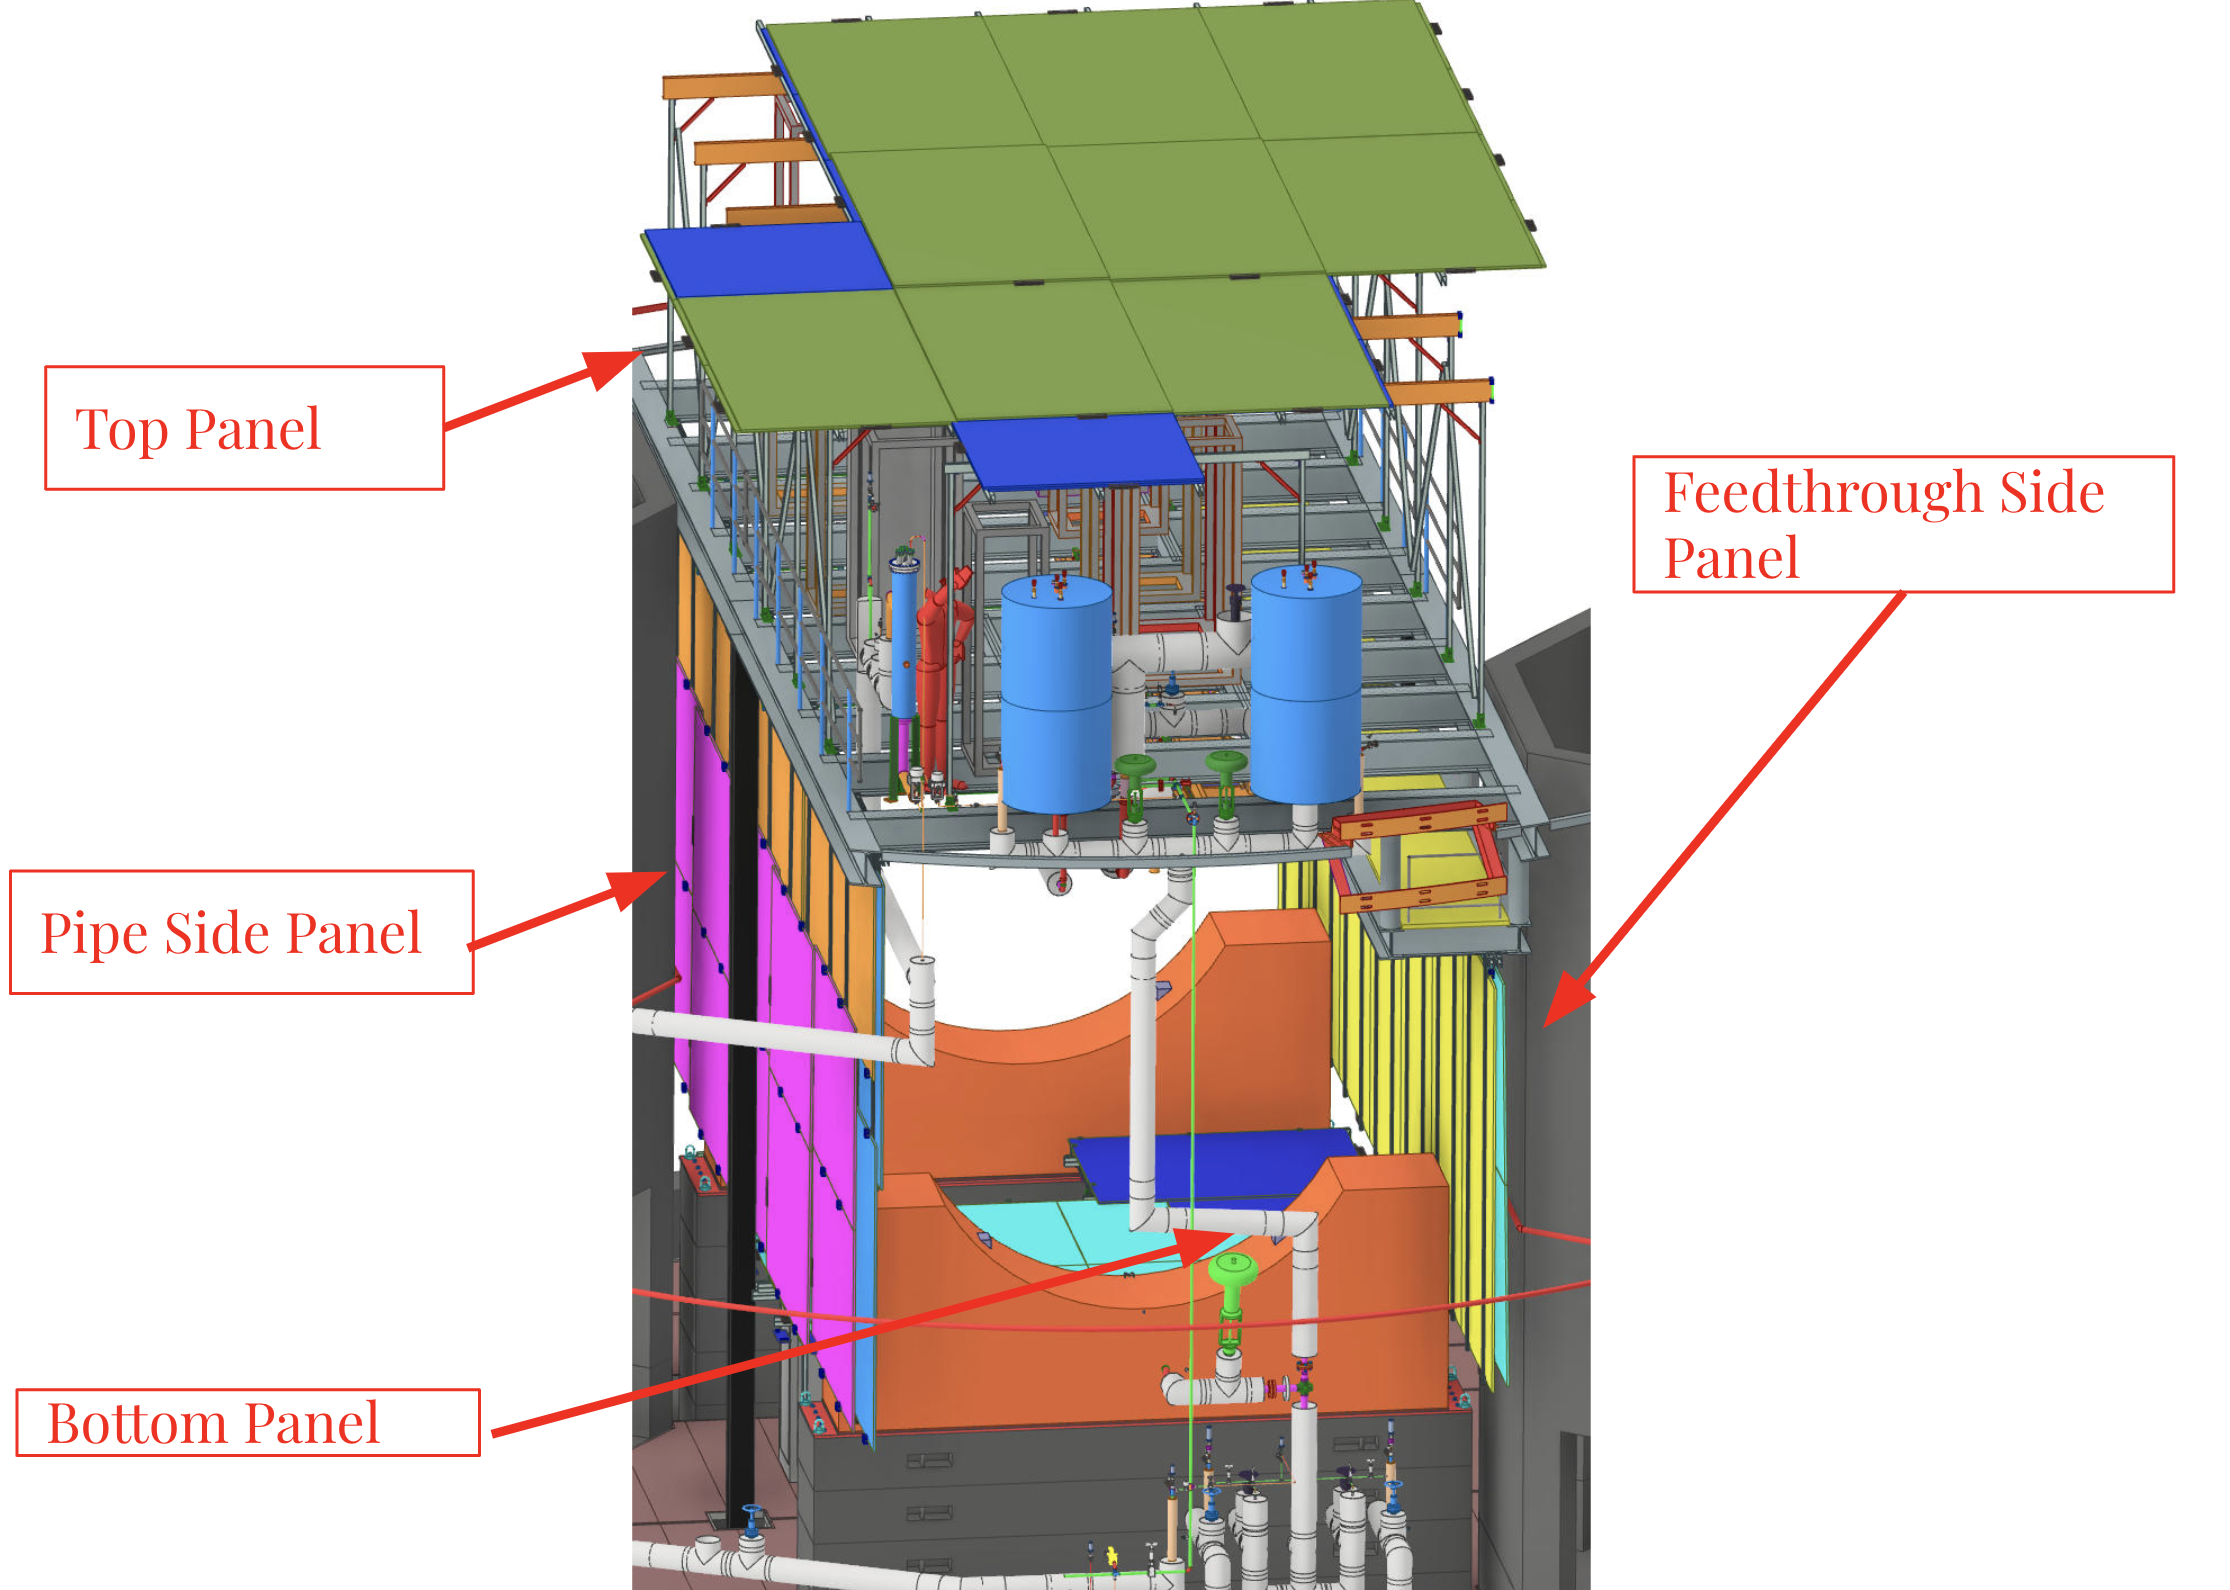
\includegraphics[scale=0.3]{images/CRTScheme}
\caption{Technical drawing of the CRT modules' position in LArTF.}
\label{fig:CRT}
\end{figure}

\subsection{POTs with good CRT information}
Data from November 30th 2017 and run number greater than 14114 are the ones deemed usable for physics analysis at this time. The total number of POT collected from November 30th 2017 up to June 30th 2019 is $\sim$6e20 POT.  



\subsection{CRT system stability}
Online monitoring metrics are in place to check the CRT stability at data taking, while a CRT data quality check is offered offline for the analyzers. We discuss here a measurement of CRT stability obtained with the latter framework.

\subsubsection{Reduced CRT Window and  Uncorrected Rate Definition}\label{sec:RateDef}
%%%%%%%%%%%%%%%%%%%%%%%%%%%%%%%%%%%%%%%%%%%%%%%%%%%%%%%%%%%%%%%%%%%%%%%%%%%%%%%%%
As discussed above, the CRT and TPC readouts are disjoint: data from the two systems are merged at the swizzling stage.  
The CRT reads out data continuously; at the swizzling stage, chunks of CRT readout are merged to the TPC event using the systems timestamps.
Originally, the merged CRT window for each TPC event spanned from -1.94 ms to 4.06 ms around the TPC trigger time. While analyzing data for this work, we noticed that this range is not sufficient to cover cosmic activity for the entire TPC drift time: for example, a cosmic ray crossing the TPC cathode 2.3 ms before the trigger time would be recorded in the TPC drift window, but would be missed in the CRT original readout window. This discovery led to a change in the CRT window merged with the TPC data: analyzers in MCC9.1 can enjoy a new CRT window that spans from -4.2 ms to 5.0 ms around the trigger time.

In order to avoid swizzling era confusion and  eventual inefficiencies at the window edges,  we used a CRT reduced window per event in this work, which is a consistent subset of the CRT data independent of the swizzling time. We define the reduced CRT window as the CRT data between -1.5 ms to 3.5 ms, see Figure \ref{fig:ReadOutWindow}. 


\begin{figure}[h!]
\centering
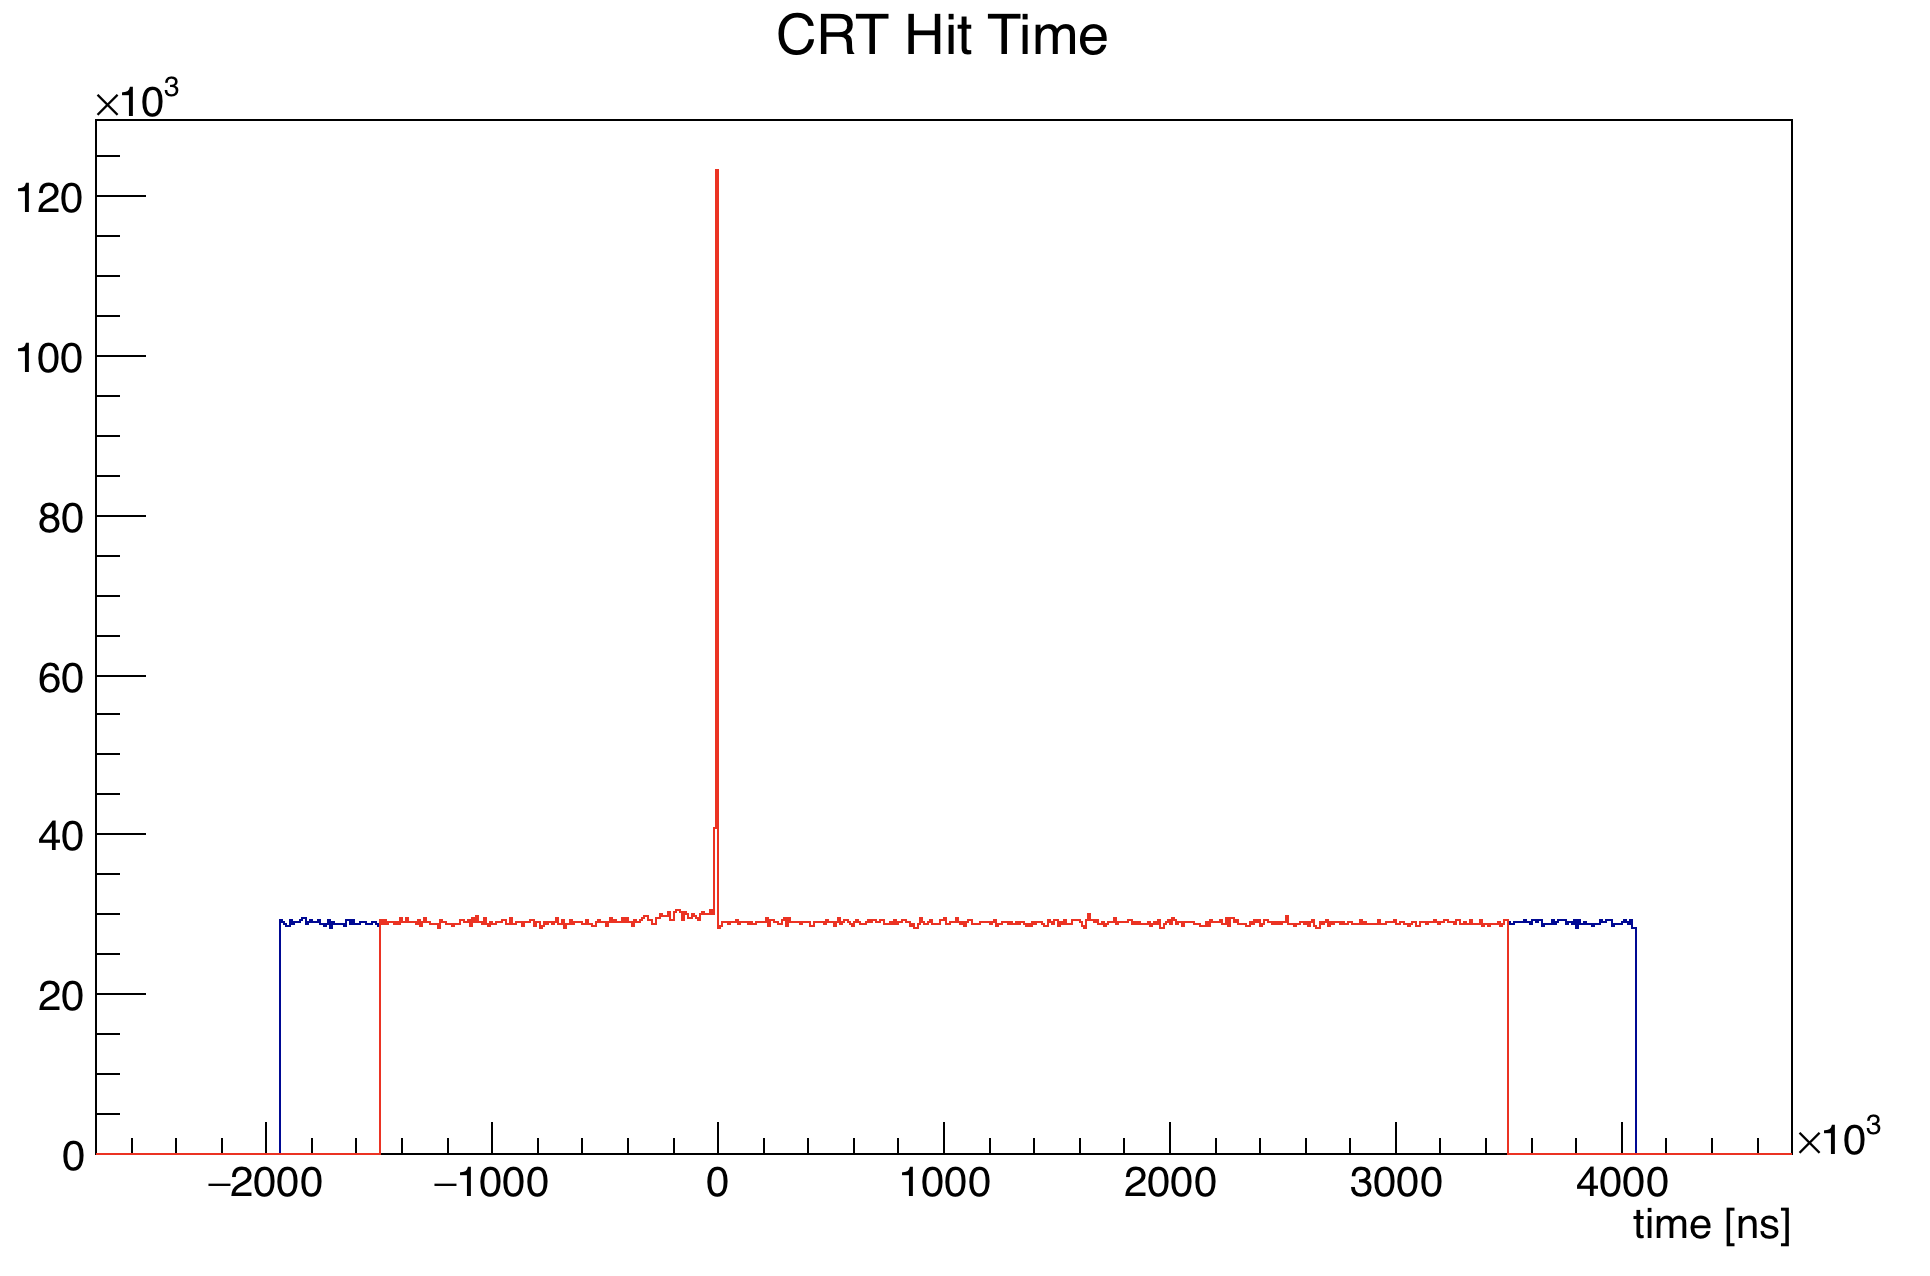
\includegraphics[scale=0.4]{images/window.png}
\caption{CRT readout window in blue, CRT reduced window in red for an arbitrary number of dates in 2018. Data showed here were merged with the original readout window.}
\label{fig:ReadOutWindow}
\end{figure}


We define the uncorrected rate as the ratio between the number of CRT hits in the reduced window and the number of considered events. We calculate the uncorrected rate on each module individually each day. 
Figure \ref{fig:count} shows number of CRT hits in the reduced window for module 11 on 01-01-2018. The integral of this distribution is 19480 hits; since the number of analyzed events that day was 13588, the uncorrected rate is 1.433 $\pm$ 0.016, where the statistical uncertainty is calculated by summing in quadrature the relative poissonian uncertainty on the numerator and denominator.

\begin{figure}[h!]
\centering
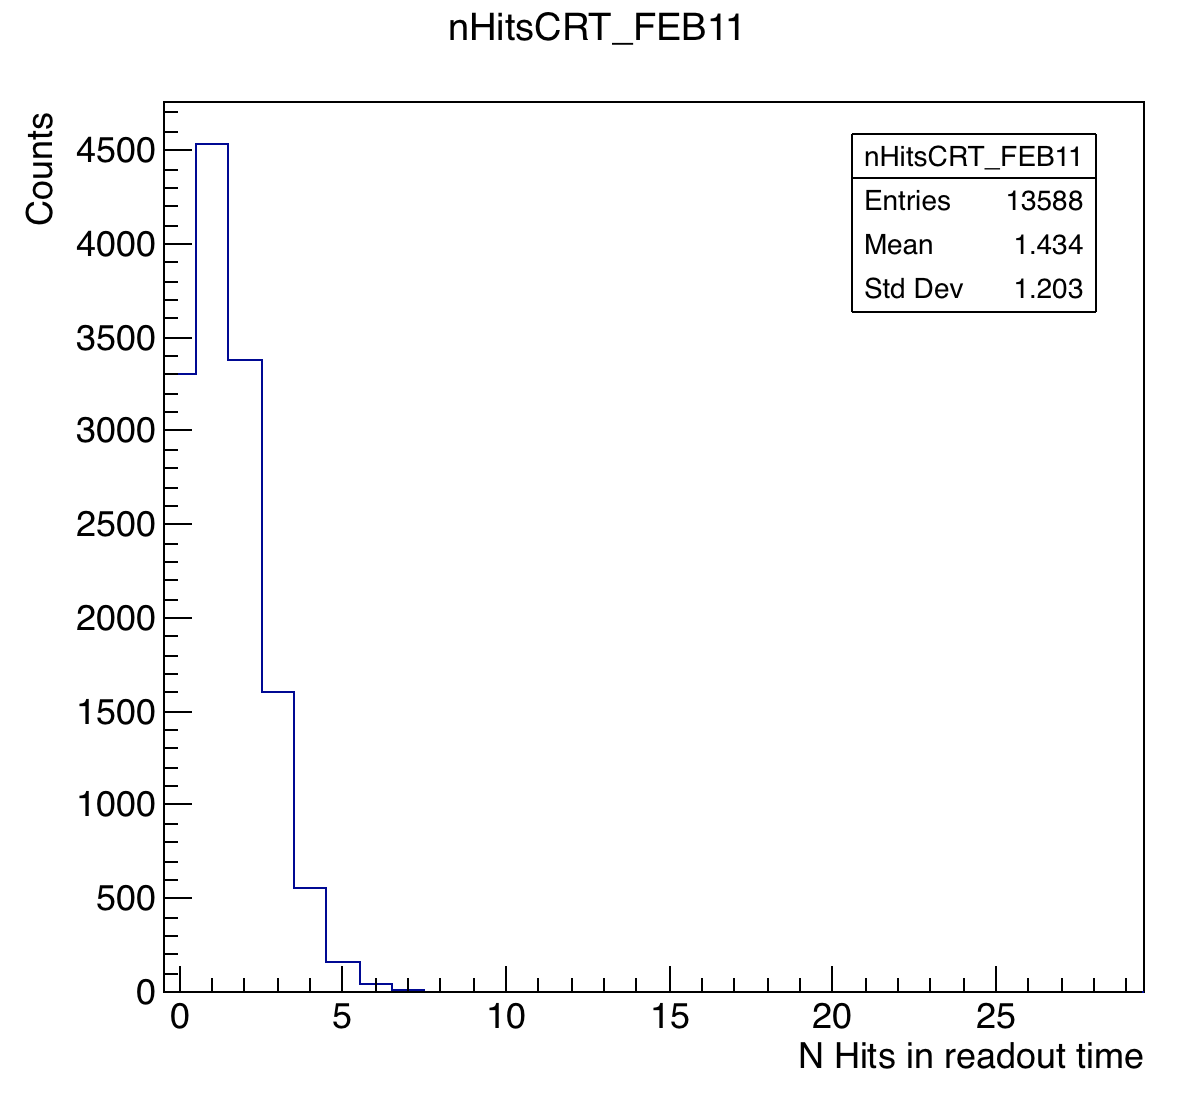
\includegraphics[scale=0.4]{images/count.png}
\caption{CRT hit count on module 11 for 01-01-2018.}
\label{fig:count}
\end{figure}
\clearpage


We analyzed the first two dates of the month for 2018 when BNBExternal data was available. 
As an example, we show the trend for Module 11 in Figure \ref{Annual11_ex}. The blue dotted line represents the average rate for BNBExt; the blue solid lines represents three standard deviations from the mean. All the dates are within three standard deviation from the mean. Analogous plots have been produced for the other 72 modules, leading to the same conclusions regarding the system stability.

\begin{figure}[h!]
\centering
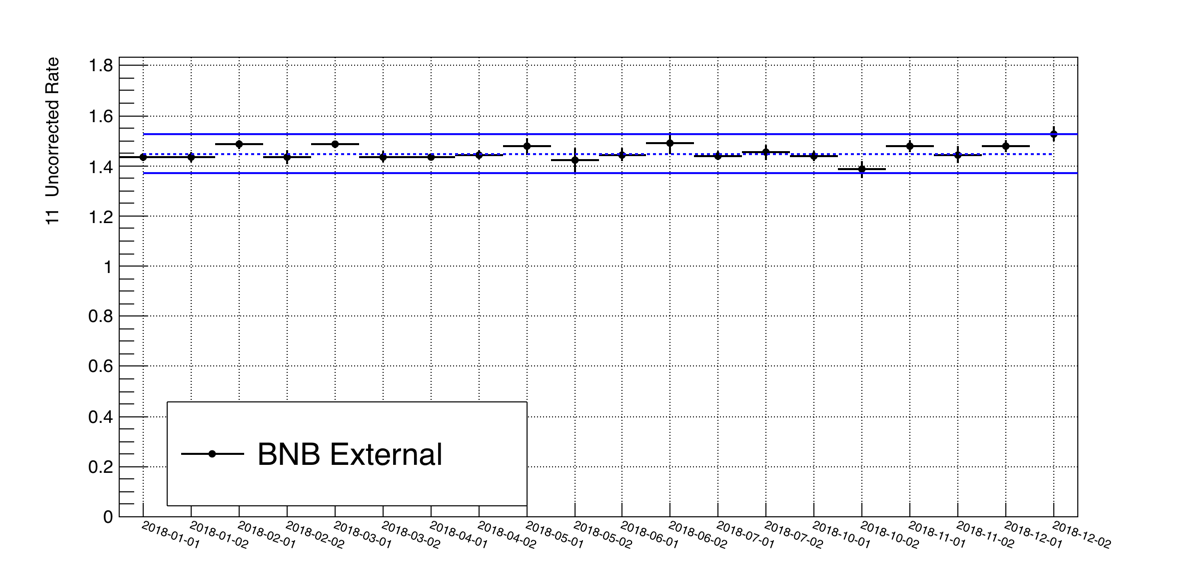
\includegraphics[scale=0.4]{images/hHitsOverEvt_FEB_11.png}
\caption{Uncorrected rate for module 11, 2018 trend: all dates are acceptable.}
\label{Annual11_ex}
\end{figure}


We note here that two hardware changes have happened during the data period deemed usable for physics analysis: a shortening of the CRT run length and the loss of a CRT strip in the top panel. Even if these changes only marginally affect the performances of the CRT, analyzers should be aware of these details when handling CRT data.
%\subsubsection{Shortening of CRT runs}
%\subsubsection{Loss of one top strip}



\section{CRT cuts: CRT Veto and Distance Tagger}\label{sec:Cuts}
In this section, we define what we mean by  CRT Veto and Distance Tagger cuts.
\subsection{CRT Veto}\label{sec:VetoCuts}
\subsection{Distance Tagger}\label{sec:DistCuts}

\newpage
\section{Rejection Power and Signal Efficiency}\label{sec:RejectionAndEff}
Since the CRT Distance Tagger requires the presence of a reconstructed neutrino vertex, we chose the pandora workflow to benchmark the performances of the CRT cuts in a electron neutrino search. These tools are easily exportable to different workflows, but in this work, we implemented the CRT Veto and CRT Distance Tagger within the pandora preselection stage. The evaluation of the pandora performances in electron neutrino searches is beyond the scope if this work: albeit wildly used, the pandora toolkit is still under development. Thus, we draw no conclusions regarding this toolkit, we disentangle the CRT  and pandora effects when possible and we present a performance assessment relative to this toolkit.\\

We start with a simple selection cut table. We are reporting here the passing rates for each cut applied to three different samples:  BNB External,  BNB Run 3 (open 1e19) and the $\nu_e$ overlay Sample. For each sample, Table \ref{tab:PS} shows the number of events passing a given cut and the  passing rate relative to the previous stage; the total passing rate without CRT cuts and with CRT cuts is shown in the last two rows.

The interpretation of the effect of the CRT cuts on the BNB External is straightforward. Since no neutrinos are present in the BNB external sample, all events that pass a selection are to be considered background.  The rejection power of cosmic background is 79\% without the use of CRT information and increases to 94\% with the use of the CRT information.

The interpretation of the effect of the CRT cuts on the $\nu_e$ overlay sample is more complex and needs to be broken down into the effect of the CRT Veto and the CRT Distance cut separately.  
As a preamble, we should note that we require that each event in our overlay sample contains an electron neutrino whose interaction is generated in the TPC active volume; no requirement is set on the containment of the charge particles produced in the interaction. Given this premise, the interpretation of the effect of the CRT Veto is, again, straightforward. Since all events include a $\nu_e$ interaction in the sample, all events rejected by the CRT Veto are to be considered an inefficiency.  Thus, the CRT Veto efficiency on electron neutrinos is overall 95\%. Figure \ref{fig:VetoE} shows the CRT Veto efficiency as a function of the true neutrino energy for true neutrino energies smaller than 2 GeV;  for true neutrino energies smaller than 700 MeV, the CRT Veto efficiency is greater than 96\%. 

Understanding the signal efficiency for the CRT Distance Tagger is more complicated, since the effect of the tagger is coupled with the identification of the vertex by the pandora framework. The last column of  Table \ref{tab:PS} shows a 7\% event reduction when applying the CRT Distance cut to the identified pandora neutrino vertex. However, there is no guarantee that pandora identifies the true neutrino activity: we just know a neutrino was reconstructed in the event.
If we want to understand the efficiency of the CRT Distance Tagger on the $\nu_e$ sample, we need to require that pandora identifies  the true neutrino vertex first. We crudely check for truth matching by requiring that the distance between the true neutrino vertex and the reconstructed neutrino vertex is less than 14 cm: these are legitimate signal events, that we use as denominator to calculate the CRT Distance Tagger efficiency on the $\nu_e$ sample.  Under this signal definition, Figure \ref{fig:DistanceE} shows the CRT Distance Tagger efficiency as a function of the true neutrino energy for true neutrino energies smaller than 2 GeV;  for true neutrino energies smaller than 700 MeV, the CRT Veto efficiency is greater than 97\%. Using the same truth matching definition, we can now estimate the rejection power of CRT Distance Tagger for the cases where a true $\nu_e$ is generated in the event, but pandora mis-identifies cosmic activities as the neutrino interaction. For this study, we select events such that the distance between the true neutrino vertex and the reconstructed neutrino vertex is greater than 14 cm: for simplicity we flag all these events as background. We then apply the CRT Distance cut. Unsurprisingly, 19\% percent of mis-identified neutrino interactions are removed by the CRT Distance tagger in the $\nu_e$ overlay sample; this is the same rejection power of the CRT Distance Cut on the BNB External, in fact we are correcting the same type of pandora misidentification.



\begin{table}[h]
\begin{tabular}{ c || c | c || c | c || c | c || }
\cline{2-7}
                                            & \multicolumn{2}{c||}{BNB External} & \multicolumn{2}{c||}{BNB Run 3 1e19} & \multicolumn{2}{c||}{$\nu_e$ overlay} \\ \cline{2-7} 
                                            & N evts        & Relative PS       & N evts         & Relative PS        & N evts       & Relative PS       \\ \hline
\multicolumn{1}{|l||}{Common Optical Filter}  & 56435         &                   & 35050          &                    & 150384       &                   \\ \hline
\multicolumn{1}{|l||}{CRT Veto}                       & 33330         & 59\%          & 22040          & 63\%               & 143227       & 95\%              \\ \hline
\multicolumn{1}{|l||}{Pandora Reco Neutrino} & 4587          & 14\%           & 5576           & 25\%              & 122390       & 85\%              \\ \hline
\multicolumn{1}{|l||}{CRT Distance}                & 3730          & 81\%            & 4861           & 87\%              & 114123       & 93\% ($>$96\%)              \\ \hline \hline 
\multicolumn{1}{|l||}{Total Passing Rate w/o CRT}    &         \multicolumn{2}{c||}{ 21\%}    &   \multicolumn{2}{c||}{28\%}  & \multicolumn{2}{c||}{85\%}\\ \hline
\multicolumn{1}{|l||}{Total Passing Rate w/ CRT}       &                 \multicolumn{2}{c||}{6\%}      & \multicolumn{2}{c||}{14\%}     &  \multicolumn{2}{c||}{76\% }   \\ \hline
\end{tabular}
\caption{Passing rates for $\nu_e$ Preselection on BNB External, BNB and $\nu_e$ overlay Samples.}
\label{tab:PS}
\end{table}


\begin{figure}[h!]
\centering
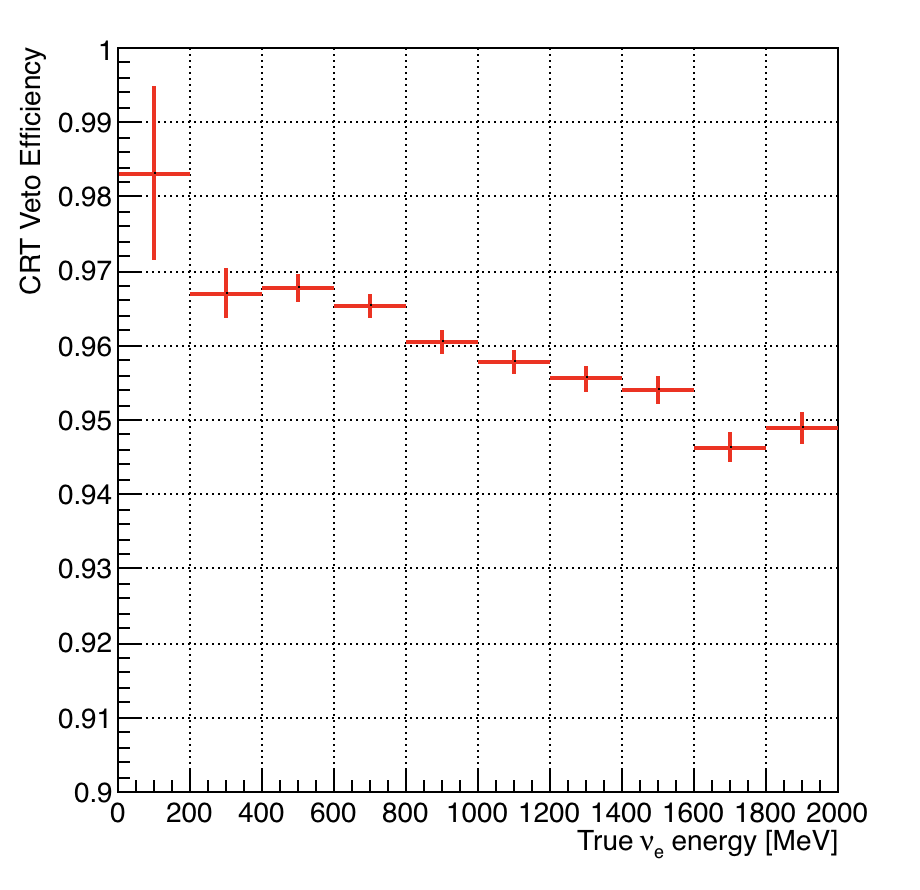
\includegraphics[scale=0.4]{images/CRTVetoEfficiency}
\caption{CRT Veto efficiency as a function of true neutrino energy in the low energy region.}
\label{fig:VetoE}
\end{figure}

\begin{figure}[h!]
\centering
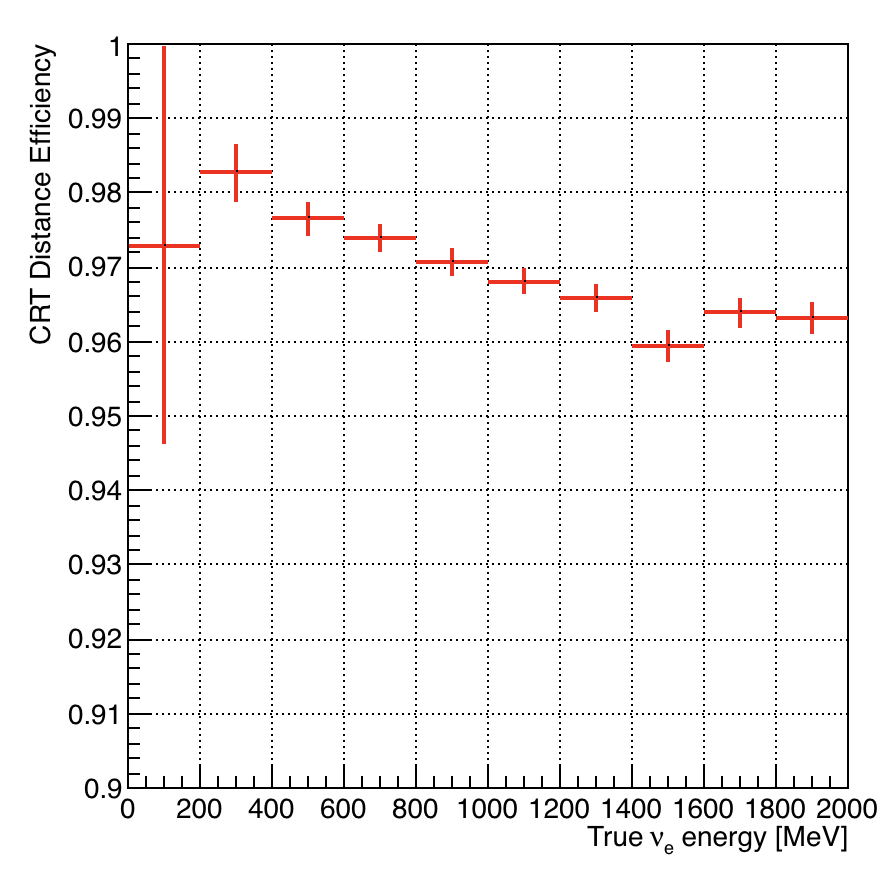
\includegraphics[scale=0.4]{images/CRTDistanceEfficiency}
\caption{CRT Distance Tagger efficiency as a function of true neutrino energy in the low energy region.}
\label{fig:DistanceE}
\end{figure}


\section{Comparison of Cutflow Significance}\label{sec:Significance}
\section{Conclusions}\label{sec:Conclusions}